% ==========================================================
% 付録J 演習問題解答
% ==========================================================
\chapter{演習問題解答}\label{app:J}

% 解答見出し用マクロ（この付録専用）
%   \appJsol{I-3-2} → 「問題 I.3.2 の解答」（問題へのリンク付き）
\newcommand{\appJsol}[1]{%
  \par\bigskip\noindent\phantomsection\label{sol:#1}%
  \textbf{\hyperref[prob:#1]{問題\,\ref*{prob:#1}}\ の解答}\par\nopagebreak\smallskip\noindent}

\begin{chapterlead}
付録Iの演習問題の解答を、種別ごとに J.1（基礎）、J.2（証明）、J.3（計算）、J.4（発展）にまとめる。各節の中では問題番号順に並べた。解答の見出しをクリックすると問題に戻る。特に断らない限り、付録Iと同じく $k$ は標数 $0$ の代数閉体である。
\end{chapterlead}

% ==========================================================
\section{基礎演習の解答}

\appJsol{I-1-1}
$g=0$ より $x=1$。これを $f$ に代入すると $1+y^2-1=y^2=0$ なので $y=0$。よって $\Zero(f,g)=\{(1,0)\}$ の $1$ 点である。

幾何学的には、直線 $x=1$ は円 $x^2+y^2=1$ の点 $(1,0)$ における接線である。直線を $x=1-\delta$ と少しずらすと $y^2=2\delta-\delta^2$ となり、$\delta>0$ では $2$ つの交点 $y=\pm\sqrt{2\delta-\delta^2}$ が現れ、$\delta\to0$ でそれらが $1$ 点に合流する。代数的には、$x=1$ を代入した $1$ 変数多項式 $y^2$ が $y=0$ を $2$ 重根にもつことに対応する。したがって交点は重複度 $2$ で数えるのが自然であり、こう数えると「$2$ 次曲線と直線の交点数は $2$」という Bézout の定理と整合する。

\appJsol{I-1-2}
$5=(2+i)(2-i)$ である。$N(2\pm i)=5$ は素数であり、$N$ は乗法的なので、$2\pm i=\alpha\beta$ ならば $N(\alpha)N(\beta)=5$ からどちらかのノルムは $1$、すなわち単元（$\pm1,\pm i$）である。よって $2\pm i$ は既約元であり、$5=(2+i)(2-i)$ が既約分解である（$2-i$ は $2+i$ の単元倍ではない：$(2+i)\cdot\{\pm1,\pm i\}=\{\pm(2+i),\ \pm(-1+2i)\}$）。

$5\Z[i]$ が素イデアルでないこと：$(2+i)(2-i)=5\in5\Z[i]$ だが、もし $2+i\in5\Z[i]$ なら $2+i=5\gamma$ で $5=N(2+i)=25N(\gamma)$ となり矛盾。同様に $2-i\notin5\Z[i]$。よって $5\Z[i]$ は素イデアルでない。（$\Z$ では素数でも $\Z[i]$ では「分解」する。付録の問題 I.10.4 も参照。）

\appJsol{I-2-1}
評価写像 $k[x,y]\to k$, $f\mapsto f(0,0)$ は全射で、核は $(x,y)$ である（$f-f(0,0)\in(x,y)$ であるから）。よって $k[x,y]/(x,y)\cong k$ は体であり、$(x,y)$ は極大イデアル。

同様に $k[x,y]\to k[y]$, $f\mapsto f(0,y)$ は全射で核は $(x)$ なので $k[x,y]/(x)\cong k[y]$。これは整域だが体ではない（$y$ は可逆でない）。よって $(x)$ は素イデアルだが極大ではない。実際 $(x)\subsetneq(x,y)$。

図形としては $\Zero(x)$ は $y$ 軸（直線）、$\Zero(x,y)$ は原点（$1$ 点）であり、$(x)\subset(x,y)$ に対して $\Zero(x)\supset\Zero(x,y)$ と包含が逆転している。

\appJsol{I-3-5}
\begin{enumerate}
  \item $\Zero(x^2)=\{0\}$ であり、$\Ideal(\{0\})=\{f\mid f(0)=0\}=(x)$。$x\notin(x^2)$ なので $(x)\neq(x^2)$。一方 $\sqrt{(x^2)}=(x)$ であるから、$\Ideal(\Zero(x^2))=\sqrt{(x^2)}$ は零点定理の主張そのものである。零点集合は「重複度」の情報 ($x^2$ の $2$ 重根) を忘れてしまう。
  \item $x,y\in\R$ なら $x^2+y^2+1\geq1>0$ なので $\Zero(x^2+y^2+1)=\emptyset$。一方、$(x^2+y^2+1)$ の元は $x^2+y^2+1$ の倍数で、$0$ でなければ次数が $2$ 以上なので $1$ を含まず、$(x^2+y^2+1)\neq\R[x,y]$。弱零点定理「$\Zero(I)=\emptyset\Rightarrow I=(1)$」は $\R$ 上では成り立たない。$\C$ 上では $\Zero(x^2+y^2+1)$ は空でない（例えば $(i,0)$）。
\end{enumerate}

\appJsol{I-4-1}
$k[x]$ は PID なので、任意のイデアルは $(f)$ と書ける。$f=0$ なら $\Zero(f)=\A^1$、$f$ が $0$ でない定数なら $\emptyset$、それ以外なら $\Zero(f)$ は $f$ の根全体で、高々 $\deg f$ 個の有限集合である。逆に有限集合 $\{a_1,\dots,a_m\}=\Zero\bigl(\prod(x-a_i)\bigr)$ は閉集合。

$k$ は代数閉体なので無限集合である。空でない開集合は有限集合の補集合なので、$2$ つの空でない開集合 $U,V$ について $U\cap V$ も有限集合の補集合であり空でない。よって相異なる $2$ 点を交わらない開近傍で分離できず、Hausdorff でない。

\appJsol{I-5-1}
$\Phi:k[x,y]\to k[x]$ を $x\mapsto x$, $y\mapsto x^2$ で定める。$\Phi$ は全射で、$y-x^2\in\Ker\Phi$。逆に $f\in k[x,y]$ に対し $y=x^2+(y-x^2)$ を代入して展開すると $f(x,y)=f(x,x^2)+(y-x^2)h(x,y)$ と書けるので、$\Phi(f)=f(x,x^2)=0$ なら $f\in(y-x^2)$。よって $\Ker\Phi=(y-x^2)$ で、$k[x,y]/(y-x^2)\cong k[x]$。

対応する多様体の同型は $\A^1\to C$, $t\mapsto(t,t^2)$ と、その逆 $C\to\A^1$, $(x,y)\mapsto x$ である。

\appJsol{I-6-1}
$a/b\in\Z_{(p)}$（$p\nmid b$、既約分数とする）が単元であることと $b/a\in\Z_{(p)}$、すなわち $p\nmid a$ は同値である。よって非単元全体は $\{a/b\mid p\mid a\}=p\Z_{(p)}$ であり、これはイデアルをなす。非単元全体がイデアルをなす環は局所環であり、そのイデアルが唯一の極大イデアルである（任意の真のイデアルは非単元からなるので $p\Z_{(p)}$ に含まれる）。

剰余体は $\Z_{(p)}/p\Z_{(p)}\cong\F_p$（$a/b\mapsto a\,b^{-1}\bmod p$）。幾何学的には $\Z_{(p)}$ は $\Spec\Z$ の点 $(p)$ の「近傍」の関数環で、剰余体は「点 $(p)$ での値」が住む体である。

\appJsol{I-8-1}
$y=x^2$ は $2$ 次なので、同次化は $yz=x^2$。無限遠直線 $z=0$ との交わりは $x^2=0$、すなわち $[0:1:0]$ の $1$ 点（重複度 $2$）のみ。したがって射影閉包 $\overline{C}=\Zero(yz-x^2)$ は放物線に $1$ 点 $[0:1:0]$ を付け加えたもので、これは非退化な $2$ 次曲線（$\PP^1$ に同型）である。放物線の $2$ つの「腕」が $y$ 軸方向の無限遠点 $1$ 点で閉じている。

\appJsol{I-9-2}
\begin{enumerate}
  \item $U_1=(0,1)$, $U_2=(2,3)$, $U=U_1\cup U_2$ とし、$a\neq b\in A$ をとる（$A\neq0$ なのでとれる；$a=0$, $b\neq0$ など）。$s_1=a\in A_{\mathrm{pre}}(U_1)$, $s_2=b\in A_{\mathrm{pre}}(U_2)$ は $U_1\cap U_2=\emptyset$ 上で（$A_{\mathrm{pre}}(\emptyset)=0$ なので）一致する。しかし $s\in A_{\mathrm{pre}}(U)=A$ で $s|_{U_1}=a$, $s|_{U_2}=b$ となるものは、制限が恒等写像なので $s=a=b$ となり存在しない。貼り合わせ公理が破れる。
  \item 局所定数関数 $U\to A$ は各連結成分上で定数なので、$\underline{A}\bigl((0,1)\cup(2,3)\bigr)\cong A\times A$。一般に $\underline{A}(U)=A^{\pi_0(U)}$（連結成分ごとに値を選ぶ）である。
\end{enumerate}

\appJsol{I-10-1}
\begin{enumerate}
  \item $k[x]/(x^2)$ の素イデアルは $x$ を含む（$x^2=0\in\p$ より）ので $(x)$ のみ。$X$ は $1$ 点 $\{(x)\}$ で、$\OO_X(X)=k[x]/(x^2)$。

  $\Spec k$ も $1$ 点で位相空間として同じだが、$\OO(\Spec k)=k$ と大域切断環が異なるのでスキームとして同型でない。関数 $x\in\OO_X(X)$ の唯一の点での値は、剰余体 $k[x]/(x)=k$ への像なので $0$ である。つまり $x$ は「すべての点で値 $0$」なのに $0$ ではない冪零元であり、スキームの関数は点での値だけでは決まらない。$X$ は「点とその点での $1$ 次の無限小方向」をもつ対象と考えられる（問題 I.10.5 参照）。
  \item $k\times k$ の素イデアルは $k\times0$ と $0\times k$ の $2$ つ（$(1,0)(0,1)=0$ より素イデアルはどちらかの成分を含む）。$\Spec(k\times k)$ は $2$ 点からなる離散空間で、$\Spec k\sqcup\Spec k$ に等しい。
\end{enumerate}

\appJsol{I-11-1}
$U_0\cap U_1=\{z_0z_1\neq0\}$ 上で $w=z_0/z_1=1/z$。$z\mapsto 1/z$ は $\C^*\to\C^*$ の正則写像で、逆写像も同じ形なので双正則である。$\varphi_0:U_0\to\C$, $[z_0:z_1]\mapsto z$ と $\varphi_1:U_1\to\C$, $[z_0:z_1]\mapsto w$ は同相写像であり、座標変換 $\varphi_1\circ\varphi_0^{-1}(z)=1/z$（$z\neq0$）が正則なので、$\{(U_0,\varphi_0),(U_1,\varphi_1)\}$ は正則アトラスであり $\C P^1$ は $1$ 次元複素多様体である。$U_0\cong\C$ に $1$ 点 $[0:1]$（$z=\infty$）を付け加えたものなので、$\C P^1$ は Riemann 球面にほかならない。

\appJsol{I-12-2}
重みの和はそれぞれ（1）$8$、（2）$6$、（3）$18$、（4）$8$。よって（1）（2）（3）は $d=\sum w_i$ を満たし Calabi--Yau 条件を満たす。（4）は $d=10>8$ で、$K_X=\OO_X(d-\sum w_i)=\OO_X(2)$ は豊富であり、一般型の $3$ 次元多様体になる（CY ではない）。

（1）について、$\PP(1,1,1,1,4)$ の次数 $8$ の多項式には単項式 $x_5^2$（重み $4\cdot2=8$）が含まれ、一般の超曲面ではその係数 $c$ は $0$ でない。点 $[0:0:0:0:1]$ では多項式の値は $c\neq0$ なので、一般の $8$ 次超曲面はこの特異点を通らない。したがって準滑らかな一般の $8$ 次超曲面は実際に滑らかな CY $3$ 次元多様体である。

\appJsol{I-13-1}
$\Lambda_{\tau+1}=\Z+\Z(\tau+1)$ は $1$ と $\tau$ を含み、逆に $\Lambda_\tau$ は $1,\tau+1$ を含むので $\Lambda_{\tau+1}=\Lambda_\tau$。

また $\tau\cdot\Lambda_{-1/\tau}=\Z\tau+\Z(-1)=\Lambda_\tau$。よって $\lambda=\tau$ として $\Lambda_\tau=\lambda\Lambda_{-1/\tau}$。

$\C/\Lambda\to\C/\lambda\Lambda$, $z\mapsto\lambda z$ は複素トーラスの同型なので、$\C/\Lambda_\tau$ の同型類は $T:\tau\mapsto\tau+1$ と $S:\tau\mapsto-1/\tau$ の作用で不変である。$\SL(2,\Z)$ は $S,T$ で生成されるので、同型類は $\SL(2,\Z)$ 軌道にしかよらない。一般に $\gamma=\begin{pmatrix}a&b\\c&d\end{pmatrix}$ に対し $(c\tau+d)\Lambda_{\gamma\tau}=\Z(a\tau+b)+\Z(c\tau+d)=\Lambda_\tau$（基底変換の行列式が $1$）と直接確かめることもできる。

\appJsol{I-14-5}
問題 I.12.4 より quintic は $\chi=-200$ なので世代数は $200/2=100$。問題 I.12.5 より $(3,3)$ 完全交差は $\chi=-144$ なので世代数は $72$。いずれも現実の $3$ 世代からはほど遠く、現実的なモデルを作るには自由な群作用による商（$\chi$ を群の位数で割る）などの工夫が必要になる。

% ==========================================================
\section{証明問題の詳細解答}

\appJsol{I-1-5}
$I\subset k[x]$ をイデアルとする。$I=0$ なら $I=(0)$。$I\neq0$ のとき、$I$ の $0$ でない元のうち次数最小のもの $f$ をとる。任意の $g\in I$ を $f$ で割って $g=qf+r$（$r=0$ または $\deg r<\deg f$）とすると、$r=g-qf\in I$。$\deg f$ の最小性より $r=0$、すなわち $g\in(f)$。よって $I=(f)$ であり、$k[x]$ は整域なので PID である。

$(x,y)\subset k[x,y]$ が単項でないこと：$(x,y)=(h)$ と仮定すると $h\mid x$ かつ $h\mid y$。$x$, $y$ は既約で互いに同伴でないので、$h$ は $0$ でない定数、つまり $(h)=(1)$。しかし $k[x,y]/(x,y)\cong k\neq0$ なので $(x,y)\neq(1)$。矛盾。

\appJsol{I-2-3}
\begin{enumerate}
  \item $\Z[x]\to\F_2$, $f\mapsto f(0)\bmod 2$ は全射環準同型で、核は $(2,x)$（$f=f(0)+xg$, $f(0)\in2\Z$ ならば $f\in(2,x)$）。よって $\Z[x]/(2,x)\cong\F_2$ は体で $(2,x)$ は極大。

  $(2,x)=(g)$ と仮定する。$2\in(g)$ より $g\mid2$ で、次数を比べて $g$ は定数、$g\in\{\pm1,\pm2\}$。$g=\pm1$ なら $(2,x)=\Z[x]$ となり極大性に反する。$g=\pm2$ なら $x\in(2)$ となるが、$x$ の係数 $1$ は偶数でないので矛盾。よって $(2,x)$ は単項でない。
  \item $\Z[x]\to\Z$, $f\mapsto f(0)$ は全射で核は $(x)$。$\Z[x]/(x)\cong\Z$ は整域だが体でないので、$(x)$ は素イデアルだが極大でない（実際 $(x)\subsetneq(2,x)$）。
\end{enumerate}

\appJsol{I-2-4}
$\p=(a)\neq0$ を素イデアル、$\m=(b)$ を $\p\subset\m$ なるイデアルとする。$a\in(b)$ より $a=bc$。$\p$ は素なので $b\in\p$ または $c\in\p$。
\begin{itemize}
  \item $b\in\p$ なら $\m=(b)\subset\p$ で $\m=\p$。
  \item $c\in\p$ なら $c=ad$ と書け、$a=bad$。$A$ は整域で $a\neq0$ なので $1=bd$、すなわち $b$ は単元で $\m=A$。
\end{itemize}
よって $\p$ と $A$ の間にイデアルはなく、$\p$ は極大（$\p\neq A$ は素イデアルの定義から）。

$\Z$, $k[x]$ は PID なので、素イデアルは $(0)$ か極大イデアルである。$\Spec$ において $(0)$ はすべての素イデアルに含まれるので閉包は全体（生成点）、極大イデアルは閉点（問題 I.10.3）である。$\Spec\Z=\{(0)\}\cup\{(p)\mid p\text{ 素数}\}$、$\Spec k[x]=\{(0)\}\cup\{(x-a)\mid a\in k\}$（$k$ は代数閉体）。

\appJsol{I-3-2}
$J=(y-x^2,\ z-x^3)$ とおく。$J\subset\Ideal(C)$ は明らか。逆を示す。任意の $f\in k[x,y,z]$ について、$y=x^2+(y-x^2)$, $z=x^3+(z-x^3)$ を代入して展開すれば
\[
  f(x,y,z)=f(x,x^2,x^3)+(y-x^2)\,h_1+(z-x^3)\,h_2\qquad(h_1,h_2\in k[x,y,z])
\]
と書ける。$f\in\Ideal(C)$ なら、すべての $t\in k$ に対し $f(t,t^2,t^3)=0$。$1$ 変数多項式 $g(x)=f(x,x^2,x^3)$ は無限個の根をもつ（$k$ は無限体）ので $g=0$。よって $f\in J$。

$C=\Zero(J)$ も成り立つ：$(a,b,c)\in\Zero(J)$ なら $b=a^2$, $c=a^3$ で $t=a$ とすればよい。したがって $C$ は代数的集合であり、$k[C]=k[x,y,z]/J\cong k[x]$（上の分解より $f\mapsto f(x,x^2,x^3)$ が同型を与える）。$k[t]$ は整域なので $C$ は既約である。

\appJsol{I-3-4}
\textbf{$\Zero(I)\cup\Zero(J)=\Zero(IJ)=\Zero(I\cap J)$.}
$IJ\subset I\cap J\subset I$ なので（イデアルが小さいほど零点集合は大きい）
$\Zero(I)\subset\Zero(I\cap J)\subset\Zero(IJ)$。同様に $\Zero(J)\subset\Zero(I\cap J)$。よって
$\Zero(I)\cup\Zero(J)\subset\Zero(I\cap J)\subset\Zero(IJ)$。

残りは $\Zero(IJ)\subset\Zero(I)\cup\Zero(J)$。$P\in\Zero(IJ)$ かつ $P\notin\Zero(I)$ とすると、$f(P)\neq0$ なる $f\in I$ がある。任意の $g\in J$ について $fg\in IJ$ なので $f(P)g(P)=0$、よって $g(P)=0$。ゆえに $P\in\Zero(J)$。

\textbf{$\bigcap\Zero(I_\lambda)=\Zero(\sum I_\lambda)$.}
各 $\lambda$ について $I_\lambda\subset\sum I_\lambda$ なので $\Zero(\sum I_\lambda)\subset\Zero(I_\lambda)$。逆に $P\in\bigcap\Zero(I_\lambda)$ とすると、$\sum I_\lambda$ の元は有限和 $f_1+\dots+f_m$（$f_j\in I_{\lambda_j}$）であり、$P$ で $0$ になる。よって等号が成り立つ。

この結果は、代数的集合の全体が有限和と任意の共通部分で閉じていること、すなわち Zariski 位相の閉集合系の公理を満たすことを示している。

\appJsol{I-4-2}
積位相の基本開集合は $U\times V$（$U,V$ は $\A^1$ の開集合）であり、その補集合は
\[
  (\A^1\times\A^1)\setminus(U\times V)=\bigl((\A^1\setminus U)\times\A^1\bigr)\cup\bigl(\A^1\times(\A^1\setminus V)\bigr).
\]
$U,V\neq\emptyset$ なら $\A^1\setminus U$, $\A^1\setminus V$ は有限集合（問題 I.4.1）なので、これは有限個の「縦線」$\{a\}\times\A^1$ と「横線」$\A^1\times\{b\}$ の和集合である。積位相の閉集合はこのような集合（と全体）の共通部分なので、全体でない閉集合 $Z$ は、ある空でない $U\times V$ の補集合に含まれる、すなわち有限個の縦線と横線の和に含まれる。

対角線 $\Delta=\{(t,t)\}$ は、各縦線・横線と $1$ 点でしか交わらないので、有限個の縦線・横線の和に含まれる $\Delta$ の点は有限個である。$k$ は無限体なので $\Delta$ は無限集合であり、どの有限個の縦線・横線の和にも含まれない。よって $\Delta$ は積位相で閉でない。一方 $\Delta=\Zero(x-y)$ は $\A^2$ の Zariski 位相で閉である。ゆえに $2$ つの位相は異なる（Zariski 位相のほうが真に細かい）。

\appJsol{I-4-3}
\textbf{稠密性.} $U\neq\emptyset$ を開集合とし、$\overline{U}$ をその閉包とする。$X=\overline{U}\cup(X\setminus U)$ は $2$ つの閉集合の和である。$X$ は既約なので $X=\overline{U}$ または $X=X\setminus U$。後者は $U\neq\emptyset$ に反するので $X=\overline{U}$。

\textbf{既約性.} $U$ の閉集合は $Z\cap U$（$Z$ は $X$ の閉集合）の形である。$U=(Z_1\cap U)\cup(Z_2\cap U)$ とすると $X=Z_1\cup Z_2\cup(X\setminus U)$。$X$ の既約性から $X$ はこの $3$ つの閉集合のどれかに等しく、$X\setminus U\neq X$ なので $X=Z_1$ または $X=Z_2$。よって $U=Z_1\cap U$ または $U=Z_2\cap U$ であり、$U$ は既約（$U\neq\emptyset$ も満たす）。

例えば $\A^2$ から曲線を除いた開集合は $\A^2$ で稠密である。

\appJsol{I-4-4}
$\{U_\lambda\}_{\lambda\in\Lambda}$ を $\A^n$ の開被覆とし、$U_\lambda=\A^n\setminus\Zero(I_\lambda)$ と書く。被覆であることは
\[
  \emptyset=\bigcap_\lambda\Zero(I_\lambda)=\Zero\Bigl(\sum_\lambda I_\lambda\Bigr)
\]
と同値（問題 I.3.4）。Hilbert の基底定理より $\sum_\lambda I_\lambda$ は有限生成で、各生成元は有限個の $I_\lambda$ の元の和なので、有限個の $\lambda_1,\dots,\lambda_m$ について $\sum_\lambda I_\lambda=I_{\lambda_1}+\dots+I_{\lambda_m}$。すると $\Zero(I_{\lambda_1}+\dots+I_{\lambda_m})=\emptyset$、すなわち $U_{\lambda_1}\cup\dots\cup U_{\lambda_m}=\A^n$。よって $\A^n$ は準コンパクトである。

（零点定理は使っていないことに注意。同じ議論で、Noether 環 $A$ の $\Spec A$ や、$\A^n$ の任意の部分空間も準コンパクトであることがわかる。）

\appJsol{I-5-2}
\begin{enumerate}
  \item $\Phi:k[x,y]\to k[t]$, $x\mapsto t^2$, $y\mapsto t^3$ を考える。像は $k[t^2,t^3]$ で、$y^2-x^3\mapsto t^6-t^6=0$。$y^2=x^3+(y^2-x^3)$ を用いて $y$ の $2$ 次以上を消すと、任意の $f$ は
  \[
    f\equiv a(x)+y\,b(x)\pmod{y^2-x^3}
  \]
  と書ける。$\Phi(a+yb)=a(t^2)+t^3b(t^2)$ で、$a(t^2)$ は偶数次の項のみ、$t^3b(t^2)$ は奇数次の項のみからなるので、これが $0$ なら $a=b=0$。よって $\Ker\Phi=(y^2-x^3)$ で、$A\cong k[t^2,t^3]$。$A$ は $k[t]$ の部分環なので整域である。
  \item $\Frac(A)=k(t)$（$t=t^3/t^2=y/x$ が分数体に含まれるので）。$t$ はモニック多項式 $T^2-t^2\in A[T]$ の根なので $A$ 上整である。しかし $k[t^2,t^3]$ は $1,t^2,t^3,t^4,\dots$ で張られる $k$ ベクトル空間で、$t\notin A$。よって $A$ は分数体の中で整閉でない。その正規化は $k[t]$ であり、これは尖点 $y^2=x^3$ の特異点解消 $\A^1\to C$ に対応する。
\end{enumerate}

\appJsol{I-5-3}
$B=k[t^2,t^3]=\{\sum c_it^i\mid c_1=0\}$ の元の次数を $k[t]$ での次数で測る。$B$ の単元は $k[t]$ の単元でもあるので $k^\times$ のみ。$B$ の定数でない元の次数は $2$ 以上である。

\textbf{$t^2$ は $B$ で既約.} $t^2=fg$（$f,g\in B$）なら $\deg f+\deg g=2$ で、次数 $1$ の元は $B$ にないので、一方は次数 $0$、すなわち単元。$t^3$ も同様に既約（$\deg f+\deg g=3$ で、$\{0,3\}$ 以外の分け方 $\{1,2\}$ は不可能）。

\textbf{$t^2$ と $t^3$ は同伴でない.} 単元は定数なので、次数の異なる $t^2$, $t^3$ は同伴でない。

したがって $t^6=t^2\cdot t^2\cdot t^2=t^3\cdot t^3$ は既約元への $2$ 通りの本質的に異なる分解をもち、$B$ は UFD でない。（$t^2\mid t^3\cdot t^3$ だが $t^2\nmid t^3$（$t^3/t^2=t\notin B$）なので、$t^2$ は既約だが素元でない、と言ってもよい。）

\appJsol{I-5-5}
$\Phi:k[x,y]\to k[x,x^{-1}]$, $x\mapsto x$, $y\mapsto x^{-1}$ は全射で、$xy-1\mapsto0$。$xy\equiv1$ を用いて単項式 $x^iy^j$ を $x^{i-j}$ または $y^{j-i}$ に置き換えれば、任意の $f$ は
\[
  f\equiv\sum_{i\geq0}a_ix^i+\sum_{j\geq1}b_jy^j\pmod{xy-1}
\]
と書け、その像 $\sum a_ix^i+\sum b_jx^{-j}$ が $0$ なら全係数が $0$。よって $\Ker\Phi=(xy-1)$ で $k[H]\cong k[x,x^{-1}]$。

$H\cong\A^1$ なら座標環も同型 $k[x,x^{-1}]\cong k[t]$ のはずである。しかし $k[x,x^{-1}]$ には定数でない単元 $x$ があるのに対し、$k[t]$ の単元は $k^\times$ のみ。単元群は環の同型で保たれ、定数（$k$ の元）も $k$ 代数の同型で保たれるので矛盾。よって $H\not\cong\A^1$。（幾何学的には $H\cong\A^1\setminus\{0\}$ であり、$x$ は「至る所消えない関数」である。）

\appJsol{I-6-3}
\textbf{(i) $\q\mapsto\varphi^{-1}(\q)$.} 素イデアルの逆像は素イデアルである。$s\in S$ なら $\varphi(s)=s/1$ は単元なので $\q$ に含まれず、$\varphi^{-1}(\q)\cap S=\emptyset$。

\textbf{(ii) $\p\mapsto S^{-1}\p$.} $\p\cap S=\emptyset$ とする。まず次を示す：
\[
  (\ast)\qquad a/s\in S^{-1}\p\ \Longrightarrow\ a\in\p.
\]
$a/s=b/t$（$b\in\p$, $t\in S$）とすると、ある $u\in S$ で $u(at-bs)=0$。よって $uta=usb\in\p$。$ut\in S$ は $\p$ に入らないので $a\in\p$。

$(\ast)$ より $1/1\notin S^{-1}\p$（$1\notin\p$）なので $S^{-1}\p$ は真のイデアル。$(a/s)(b/t)\in S^{-1}\p$ なら $(\ast)$ より $ab\in\p$ なので $a\in\p$ または $b\in\p$。よって $S^{-1}\p$ は素イデアル。また $(\ast)$ は $\varphi^{-1}(S^{-1}\p)=\p$ を意味する（$\supset$ は明らか）。

\textbf{(iii) $S^{-1}(\varphi^{-1}(\q))=\q$.} $\subset$：$a\in\varphi^{-1}(\q)$ なら $a/s=(a/1)(1/s)\in\q$。$\supset$：$a/s\in\q$ なら $a/1=(s/1)(a/s)\in\q$ なので $a\in\varphi^{-1}(\q)$、よって $a/s\in S^{-1}(\varphi^{-1}(\q))$。

(ii)(iii) より $2$ つの写像は互いに逆である。（包含関係も保つので、$\Spec S^{-1}A$ は $\Spec A$ の部分空間 $\{\p\mid\p\cap S=\emptyset\}$ と同一視できる。$S=\{f^n\}$ なら開集合 $D(f)$、$S=A\setminus\p$ なら「$\p$ を含む素イデアル全体」ではなく「$\p$ に含まれる素イデアル全体」になる。）

\appJsol{I-7-3}
$F=x^n+y^n+z^n$ とすると $F_x=nx^{n-1}$, $F_y=ny^{n-1}$, $F_z=nz^{n-1}$。$p\nmid n$ なら $n\neq0$ in $k$ なので、$F_x=F_y=F_z=0$ から $x=y=z=0$。これは $\PP^2$ の点ではない。よって $F_n$ 上（実は $\PP^2$ 全体で）偏微分が同時に消える点はなく、$F_n$ は滑らかである。（射影曲線の特異点は $F=F_x=F_y=F_z=0$ の点であり、Euler の等式 $xF_x+yF_y+zF_z=nF$ より $p\nmid n$ なら $F=0$ は偏微分の条件から従う。）

$p\mid n$ のとき、偏微分はすべて恒等的に $0$ なので、$F_n$ のすべての点が特異点である。例えば $n=p$ なら $x^p+y^p+z^p=(x+y+z)^p$ であり、$F_n$ は直線 $x+y+z=0$ を $p$ 重に数えた被約でない曲線になる。

\appJsol{I-8-5}
$Z$ を $\Zero(f)$ の $\PP^n$ での閉包とする。

\textbf{$Z\subset\Zero(f^h)$.} $f^h(1,x_1,\dots,x_n)=f(x_1,\dots,x_n)$ なので $\Zero(f^h)\cap\{x_0\neq0\}=\Zero(f)$。特に $\Zero(f)\subset\Zero(f^h)$ で、$\Zero(f^h)$ は閉集合なので $Z\subset\Zero(f^h)$。

\textbf{$\Zero(f^h)\subset Z$.} $\PP^n$ の閉集合は同次多項式の共通零点なので、$Z=\Zero(\{G\mid G\text{ は同次で }\Zero(f)\text{ 上で } 0\})$。このような $G$ をとり、$G_*=G(1,x_1,\dots,x_n)$ をその非同次化とする。$G_*$ は $\Zero(f)$ 上で $0$ なので、零点定理より $G_*\in\Ideal(\Zero(f))=\sqrt{(f)}$。$f$ は平方因子をもたないので $\sqrt{(f)}=(f)$、すなわち $G_*=fh$。

一般に、同次多項式 $G$ について $G=x_0^a\,(G_*)^h$（$a\ge 0$ は $G$ が $x_0$ で割り切れる回数）であり、また積の同次化は同次化の積 $(fh)^h=f^hh^h$ である。よって
\[
  G=x_0^a\,f^h\,h^h
\]
で $f^h\mid G$。したがって $G$ は $\Zero(f^h)$ 上で $0$ となり、$\Zero(f^h)\subset Z$。

以上より $Z=\Zero(f^h)$。（$f$ が平方因子をもつ場合も $f$ をその被約部分に置き換えれば同じ結論になる。超曲面でない場合は、生成元ごとに同次化するだけでは一般に閉包が得られず、イデアル全体の同次化が必要になる。）

\appJsol{I-9-1}
\textbf{局所性は成り立つ.} $s\in\sheaf{B}(U)$ が開被覆 $\{U_i\}$ の各 $U_i$ 上で $0$ なら、$U$ の各点で $s=0$ なので $s=0$。

\textbf{貼り合わせ公理が破れる.} $U_n=(-n,n)$ とし、$s_n=x|_{U_n}$ とする。$|s_n|<n$ なので $s_n\in\sheaf{B}(U_n)$ であり、重なりで $s_n|_{U_n\cap U_m}=s_m|_{U_n\cap U_m}$ と整合する。しかし $\{U_n\}$ は $\R$ の開被覆であり、貼り合わせた関数は $x$ そのものであって $\R$ 上で有界でない。$\sheaf{B}(\R)$ の元で各 $s_n$ に制限されるものは（局所性から一意に $x$ でなければならないので）存在しない。

有界性は「大域的な」条件であり、局所的な条件の積み重ねで表せないことが原因である。（連続関数全体の層の部分前層として、有界という条件を外せば層になる。）

\appJsol{I-9-4}
\textbf{(1)$\Rightarrow$(2).} $s_p\in\sheaf{F}_p$ を $\varphi_p(s_p)=0$ とし、$s_p$ を点 $p$ の開近傍 $U$ 上の切断 $s$ で代表させる。$\varphi_p(s_p)=(\varphi_U(s))_p=0$ なので、ある開近傍 $V\subset U$ で $\varphi_U(s)|_V=\varphi_V(s|_V)=0$。$\varphi_V$ は単射なので $s|_V=0$、したがって $s_p=0$。

\textbf{(2)$\Rightarrow$(1).} $s\in\sheaf{F}(U)$ を $\varphi_U(s)=0$ とする。各 $p\in U$ で $\varphi_p(s_p)=(\varphi_U(s))_p=0$ なので $s_p=0$。すなわち各 $p$ のある開近傍 $V_p\subset U$ で $s|_{V_p}=0$。$\{V_p\}$ は $U$ の開被覆なので、層の局所性公理から $s=0$。

（全射性については同様の同値は成り立たない。茎ごとに全射でも $\varphi_U$ は全射とは限らない。問題 I.9.5 がその例である。）

\appJsol{I-10-3}
$\Spec A$ の閉集合は $\Zero(I)=\{\q\mid\q\supset I\}$ の形である。$\p\in\Zero(I)\iff I\subset\p\iff\Zero(\p)\subset\Zero(I)$（後者の $\Rightarrow$：$\q\supset\p\supset I$。$\Leftarrow$：$\p\in\Zero(\p)$）。よって $\p$ を含むすべての閉集合の共通部分は $\Zero(\p)$ 自身であり、$\overline{\{\p\}}=\Zero(\p)$。

$\{\p\}$ が閉 $\iff\Zero(\p)=\{\p\}\iff$ $\p$ を真に含む素イデアルがない。$\p$ が極大ならこれは成り立つ。逆に $\p$ が極大でなければ、$\p\subsetneq I\subsetneq A$ なるイデアル $I$ があり、$I$ を含む極大イデアル $\m$（Zorn の補題）は素イデアルで $\p\subsetneq\m$。よって $\p$ は閉点でない。

\appJsol{I-11-2}
\begin{enumerate}
  \item $X$ をコンパクト連結複素多様体、$f$ を正則関数とする。$|f|$ は連続なので、ある点 $p$ で最大値をとる。$Z=\{x\in X\mid f(x)=f(p)\}$ は閉集合で $p\in Z$。$q\in Z$ を任意にとると、$|f|$ は $q$ でも最大値をとる。$q$ を中心とする連結な座標近傍（多重円板）において、最大値の原理（多変数でも各複素直線に制限すれば $1$ 変数の場合に帰着する）より $f$ はその近傍で定数 $f(q)=f(p)$。よって $Z$ は開集合でもある。$X$ は連結で $Z\neq\emptyset$ なので $Z=X$、すなわち $f$ は定数。
  \item $f$ を $E$ 上の正則関数とし、射影 $\pi:\C\to E$ で引き戻した $F=f\circ\pi$ を考える。$F$ は $\C$ 上の整関数で、$F(z+1)=F(z+\tau)=F(z)$ を満たす。よって $F(\C)=F(P)$（$P$ は $0,1,\tau,1+\tau$ を頂点とする閉平行四辺形）であり、$P$ はコンパクトなので $F$ は有界。Liouville の定理より $F$ は定数、したがって $f$ も定数。
\end{enumerate}

\appJsol{I-12-6}
Hodge 分解より $b_n=\sum_{p+q=n}h^{p,q}$。仮定と対称性から
\begin{align*}
  &h^{0,0}=h^{3,3}=1,\quad h^{1,0}=h^{0,1}=h^{3,2}=h^{2,3}=0,\quad h^{2,0}=h^{0,2}=h^{3,1}=h^{1,3}=0,\\
  &h^{3,0}=h^{0,3}=1,\quad h^{2,2}=h^{1,1},\quad h^{1,2}=h^{2,1}.
\end{align*}
したがって Hodge ダイヤモンドは
\[
\begin{array}{ccccccc}
 &&&1&&&\\
 &&0&&0&&\\
 &0&&h^{1,1}&&0&\\
 1&&h^{2,1}&&h^{2,1}&&1\\
 &0&&h^{1,1}&&0&\\
 &&0&&0&&\\
 &&&1&&&
\end{array}
\]
となり、$h^{1,1}$ と $h^{2,1}$ だけで決まる。Betti 数は $b_0=b_6=1$, $b_1=b_5=0$, $b_2=b_4=h^{1,1}$, $b_3=2+2h^{2,1}$ であり、
\[
  \chi=\sum_n(-1)^nb_n=1+h^{1,1}-(2+2h^{2,1})+h^{1,1}+1=2\bigl(h^{1,1}-h^{2,1}\bigr).
\]
（ミラー対称性は $h^{1,1}\leftrightarrow h^{2,1}$ の入れ替えであり、$\chi\mapsto-\chi$ となる。）

\appJsol{I-13-3}
$\Lambda_i=\Z+\Z i$ について、$i\cdot1=i$, $i\cdot i=-1$ なので $i\Lambda_i=\Lambda_i$。斉次性より
\[
  g_3(\Lambda_i)=g_3(i\Lambda_i)=i^{-6}g_3(\Lambda_i)=-g_3(\Lambda_i),
\]
よって $g_3(\Lambda_i)=0$。判別式 $g_2^3-27g_3^2$ は格子に対して $0$ にならない（$\C/\Lambda$ が滑らかな $3$ 次曲線 $y^2=4x^3-g_2x-g_3$ に対応するため）ので $g_2(\Lambda_i)\neq0$ で、$j(i)=1728g_2^3/g_2^3=1728$。

$\Lambda_\rho=\Z+\Z\rho$ について、$\rho\cdot1=\rho$, $\rho\cdot\rho=\rho^2=-1-\rho$（$1+\rho+\rho^2=0$）なので $\rho\Lambda_\rho\subset\Lambda_\rho$、同様に $\rho^{-1}=\rho^2$ を掛けても保たれるので $\rho\Lambda_\rho=\Lambda_\rho$。
\[
  g_2(\Lambda_\rho)=g_2(\rho\Lambda_\rho)=\rho^{-4}g_2(\Lambda_\rho)=\rho^{2}g_2(\Lambda_\rho)
\]
で $\rho^2\neq1$ なので $g_2(\Lambda_\rho)=0$。よって $j(\rho)=0$。

（$i$, $\rho$ は格子が非自明な回転対称性をもつ唯一の点（の $\SL(2,\Z)$ 軌道）であり、それが $j$ の特別な値に対応している。問題 I.13.5 参照。）

% ==========================================================
\section{計算問題の詳細解答}

\appJsol{I-1-3}
\begin{enumerate}
  \item $\Phi:\R[x]\to\C$, $x\mapsto i$ を考える。$a+bi=\Phi(a+bx)$ なので全射。$\Phi(x^2+1)=0$ より $(x^2+1)\subset\Ker\Phi$。$f\in\Ker\Phi$ を $x^2+1$ で割って $f=q(x^2+1)+(a+bx)$ とすると $0=\Phi(f)=a+bi$ より $a=b=0$。よって $\Ker\Phi=(x^2+1)$ で $\R[x]/(x^2+1)\cong\C$。
  \item $\C$ 上では $x^2+1=(x-i)(x+i)$ で、$(x-i)-(x+i)=-2i$ は単元なので $(x-i)+(x+i)=(1)$。中国剰余定理より
  \[
    \C[x]/(x^2+1)\cong\C[x]/(x-i)\times\C[x]/(x+i)\cong\C\times\C,\qquad f\mapsto(f(i),f(-i)).
  \]
\end{enumerate}
幾何学的には、$\C$ 上で $x^2+1=0$ は $2$ 点 $\pm i$ からなり、その座標環は「$2$ 点上の関数 $=$ 値の組」$\C\times\C$ である。$\R$ 上では実の解はないが、$\Spec\R[x]/(x^2+1)=\Spec\C$ は $1$ 点であって、$\pm i$ の $2$ 点が複素共役で $1$ 点に「束ねられた」もの（剰余体 $\C$ をもつ点）と見ることができる。

\appJsol{I-1-4}
互除法を実行する：
\begin{align*}
  x^6-1&=x^2(x^4-1)+(x^2-1),\\
  x^4-1&=(x^2+1)(x^2-1)+0.
\end{align*}
よって $\gcd(x^6-1,x^4-1)=x^2-1$ であり、第 $1$ 式より
\[
  x^2-1=1\cdot(x^6-1)+(-x^2)\cdot(x^4-1).
\]
すなわち $a=1$, $b=-x^2$。これより $x^2-1\in(x^6-1,x^4-1)$。逆に $x^2-1$ は $x^6-1$, $x^4-1$ をともに割り切るので $(x^6-1,x^4-1)\subset(x^2-1)$。ゆえに $(x^6-1,x^4-1)=(x^2-1)$。幾何学的には $\Zero(x^6-1)\cap\Zero(x^4-1)=\{\text{$6$ 乗根}\}\cap\{\text{$4$ 乗根}\}=\{\pm1\}=\Zero(x^2-1)$。

\appJsol{I-2-2}
\begin{enumerate}
  \item $x^2\in I$ なので $x\in\sqrt I$、よって $(x)\subset\sqrt I$。一方 $I\subset(x)$ で、$(x)$ は素イデアル（$k[x,y]/(x)\cong k[y]$ は整域）なので根基イデアル。よって $\sqrt I\subset\sqrt{(x)}=(x)$。ゆえに $\sqrt I=(x)$。

  （$\Zero(I)=\Zero(x)$ は $y$ 軸。$I=(x)\cap(x^2,y)$ と分解でき、$I$ は $y$ 軸に原点の「埋没成分」が付いたものである。）
  \item $(xy)^2=x^2y^2=x\cdot(xy^2)\in J$ なので $xy\in\sqrt J$。一方 $J\subset(xy)$ で、$(xy)=(x)\cap(y)$ は素イデアルの共通部分なので根基イデアル。よって $\sqrt J\subset(xy)$。ゆえに $\sqrt J=(xy)$。$\Zero(J)$ は $2$ つの座標軸の和である。
\end{enumerate}

\appJsol{I-3-1}
$(xy,xz)=(x)\cap(y,z)$ を示す。$xy,xz$ はどちらも $(x)$ と $(y,z)$ に属するので $\subset$。逆に $f\in(x)\cap(y,z)$ とすると $f=xg$。$(y,z)$ は素イデアル（$k[x,y,z]/(y,z)\cong k[x]$）で $x\notin(y,z)$ なので $g\in(y,z)$、$g=ay+bz$。よって $f=a\,xy+b\,xz\in(xy,xz)$。

したがって $X=\Zero(x)\cup\Zero(y,z)$。$\Zero(x)$ は $yz$ 平面（$\cong\A^2$）、$\Zero(y,z)$ は $x$ 軸（$\cong\A^1$）で、いずれも既約。互いに他を含まないので、これが既約分解である：
\[
  X=\underbrace{\{x=0\}}_{\text{平面}}\ \cup\ \underbrace{\{y=z=0\}}_{\text{直線}}.
\]
（次元の異なる成分をもつことに注意。問題 I.7.4 参照。）

\appJsol{I-3-3}
第 $2$ の方程式 $xz-x=x(z-1)=0$ より $x=0$ または $z=1$。
\begin{itemize}
  \item $x=0$ のとき：第 $1$ 式は $yz=0$ となり、$y=0$ または $z=0$。それぞれ $\Zero(x,y)$（$z$ 軸）、$\Zero(x,z)$（$y$ 軸）。
  \item $z=1$ のとき：第 $1$ 式は $x^2-y=0$ となり、$\Zero(y-x^2,\ z-1)$（平面 $z=1$ 上の放物線）。
\end{itemize}
よって
\[
  X=\Zero(x,y)\cup\Zero(x,z)\cup\Zero(y-x^2,\ z-1).
\]
各成分は $\A^1$ に同型（$z$ 軸、$y$ 軸、$t\mapsto(t,t^2,1)$）なので既約で、どれも他の成分に含まれない（互いに異なる既約曲線で、交わりは有限個の点：$z$ 軸と $y$ 軸は原点で、$z$ 軸と放物線は $(0,0,1)$ で交わり、$y$ 軸と放物線は交わらない）。したがってこれが既約分解である。

\appJsol{I-4-5}
$S\subset\Zero(y-x^2)=:P$ で $P$ は閉なので $\overline S\subset P$。射影 $\pi:P\to\A^1$, $(x,y)\mapsto x$ は逆写像 $x\mapsto(x,x^2)$ をもち、両方とも多項式写像なので Zariski 位相で連続、すなわち同相写像である。$\pi(S)=\Z$ は $\A^1(\C)$ の無限部分集合なので、問題 I.4.1 よりその閉包は $\A^1$。よって $S$ の $P$ での閉包は $P$ 全体であり、$P$ は閉なので $\overline S=P=\Zero(y-x^2)$。

同様に $S'=\Z\times\{0\}$ の Zariski 閉包は $x$ 軸 $\Zero(y)$ 全体である。一方 Euclid 位相では $S'$ は離散的な閉集合なので、閉包は $S'$ 自身である。Zariski 位相は非常に粗く、「無限個の点」は多項式で切り出せる最小の集合（ここでは直線全体）まで膨らんでしまう。

\appJsol{I-5-4}
\begin{enumerate}
  \item $(a,b)\in C$、すなわち $b^2=a^3$ とする。$a\neq0$ のとき、$t^2=a$, $t^3=b$ を満たす $t$ は $t=b/a$ に限る（$t=t^3/t^2$）。実際 $(b/a)^2=b^2/a^2=a^3/a^2=a$, $(b/a)^3=b\cdot(b^2/a^3)=b$。$a=0$ なら $b=0$ で $t=0$ のみ。よって $\varphi$ は全単射で、逆写像は
  \[
    \psi(a,b)=\begin{cases}b/a&(a\neq0)\\0&(a=b=0)\end{cases}
  \]
  である。
  \item $\varphi^*:k[C]=k[x,y]/(y^2-x^3)\to k[t]$ は $x\mapsto t^2$, $y\mapsto t^3$ で、問題 I.5.2 より像は $k[t^2,t^3]$。$t\notin k[t^2,t^3]$ なので $\varphi^*$ は全射でない。アフィン多様体の射 $\varphi$ が同型であることと $\varphi^*$ が環の同型であることは同値なので、$\varphi$ は同型でない。

  実際、逆写像 $\psi=y/x$ は原点で正則関数として定義されない（$y/x$ を多項式に延長できない）。$\varphi$ は尖点 $C$ の正規化（特異点解消）である。
\end{enumerate}

\appJsol{I-6-2}
$A_x\cong A[t]/(xt-1)=k[x,y,t]/(xy,\ xt-1)$。この環の中で
\[
  y=y\cdot1=y\cdot xt=t\cdot(xy)=0.
\]
したがって $k[x,y,t]/(xy,xt-1)=k[x,y,t]/(y,\ xt-1)\cong k[x,t]/(xt-1)\cong k[x,x^{-1}]$（問題 I.5.5 と同様）。

幾何学的には、$\Spec A=\Zero(xy)$ は $2$ 本の座標軸の和であり、$x$ で局所化することは開集合 $D(x)=\{x\neq0\}$ に制限することに当たる。$x\neq0$ の部分では $y=0$ でなければならないので、$D(x)$ は「$x$ 軸から原点を除いたもの」$\cong\A^1\setminus\{0\}$ であり、その座標環が $k[x,x^{-1}]$ である。$y$ 軸は丸ごと消える。

\appJsol{I-6-4}
$f=y^2-x^3-x^2$ とする。点 $P=(a,b)$ の極大イデアル $\m=(x-a,y-b)\subset k[x,y]$ について
\[
  \m_P/\m_P^2\cong\m/(\m^2+(f))
\]
である。$\m/\m^2$ は $x-a$, $y-b$ の類を基底とする $2$ 次元空間で、$f$ の類は $f$ の $P$ での $1$ 次部分 $f_x(P)(x-a)+f_y(P)(y-b)$ に等しい。
\begin{enumerate}
  \item $P=(0,0)$：$f=y^2-x^2-x^3$ は定数項・$1$ 次の項をもたず $f\in\m^2$。よって $\dim_k\m_P/\m_P^2=2$。曲線（$1$ 次元）なのに $2$ なので、原点は特異点である。
  \item $P=(-1,0)$：$f(-1,0)=0-(-1)-1=0$ で確かに $P\in C$。$u=x+1$ とおくと
  \[
    f=y^2-(u-1)^3-(u-1)^2=y^2-(u-1)^2u=y^2-u+2u^2-u^3.
  \]
  $1$ 次部分は $-u\neq0$ なので、$\m/(\m^2+(f))$ は $\langle u,y\rangle/\langle u\rangle$ で $\dim_k\m_P/\m_P^2=1$。$P$ は非特異点である。
\end{enumerate}

\appJsol{I-7-1}
$f=y^2-x^3-x^2$ とすると
\[
  f_x=-3x^2-2x=-x(3x+2),\qquad f_y=2y.
\]
$f_y=0$ より $y=0$、$f_x=0$ より $x=0$ または $x=-2/3$。
\begin{itemize}
  \item $(0,0)$：$f(0,0)=0$ で $C$ 上にある。特異点。
  \item $(-2/3,0)$：$f=-\bigl(-\tfrac{8}{27}\bigr)-\tfrac49=\tfrac{8}{27}-\tfrac{12}{27}=-\tfrac{4}{27}\neq0$ で $C$ 上にない。
\end{itemize}
よって特異点は原点のみ。原点での $f$ の最低次部分は $y^2-x^2=(y-x)(y+x)$ なので、接錐は $2$ 直線 $y=\pm x$ の和である。原点は $2$ つの枝が異なる接線で交わる通常 $2$ 重点（ノード）である。

\begin{center}
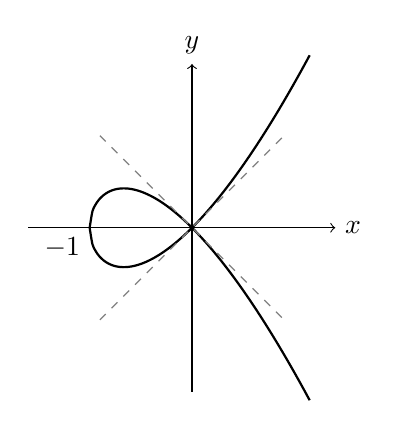
\begin{tikzpicture}[scale=1.3]
  \draw[->] (-1.6,0)--(1.4,0) node[right]{$x$};
  \draw[->] (0,-1.6)--(0,1.6) node[above]{$y$};
  \draw[thick,domain=-1:1.15,samples=80,smooth] plot ({\x},{\x*sqrt(\x+1)});
  \draw[thick,domain=-1:1.15,samples=80,smooth] plot ({\x},{-\x*sqrt(\x+1)});
  \draw[dashed,gray] (-0.9,-0.9)--(0.9,0.9);
  \draw[dashed,gray] (-0.9,0.9)--(0.9,-0.9);
  \node[below left] at (-1,0) {$-1$};
\end{tikzpicture}
\end{center}

\appJsol{I-7-2}
\begin{enumerate}
  \item $F=x^2+y^2+z^2$ の勾配は $(2x,2y,2z)$ で、$0$ になるのは原点のみ。原点は $X$ 上にあるので、$\Sing X=\{(0,0,0)\}$。
  \item 射影曲線 $Q$ の特異点は $F_x=F_y=F_z=0$ を満たす $\PP^2$ の点だが、それは $(x,y,z)=(0,0,0)$ を要求し、$\PP^2$ の点ではない。よって $Q$ は滑らかである（実際 $Q\cong\PP^1$）。
\end{enumerate}
$X$ は $Q$ のアフィン錐 $\{(x,y,z)\mid[x:y:z]\in Q\}\cup\{0\}$ であり、底 $Q$ が滑らかでも錐の頂点は特異点になる。これは $\C^2/\{\pm1\}$ の $A_1$ 特異点と同じものである。

\appJsol{I-7-4}
\begin{enumerate}
  \item 問題 I.3.1 より $X=\Zero(x)\cup\Zero(y,z)$。$\Zero(x)\cong\A^2$ は $2$ 次元、$\Zero(y,z)\cong\A^1$ は $1$ 次元。$X$ の次元は既約成分の次元の最大値なので $\dim X=2$（代数的には $\dim k[x,y,z]/(xy,xz)=2$）。
  \item 生成元 $f_1=xy$, $f_2=xz$ の Jacobi 行列は
  \[
    J=\begin{pmatrix}y&x&0\\ z&0&x\end{pmatrix}.
  \]
  Zariski 接空間の次元は $3-\rank J(P)$ である（$(xy,xz)$ は根基イデアルなので、この生成元で計算してよい）。
  \begin{itemize}
    \item $(0,0,0)$：$J=0$ で $\dim T=3$。この点を通る成分の最大次元は $2$ なので特異点。
    \item $(0,1,0)$：$J=\begin{pmatrix}1&0&0\\0&0&0\end{pmatrix}$, $\rank=1$, $\dim T=2$。平面成分のみを通り、次元 $2$ と一致するので非特異点。
    \item $(1,0,0)$：$J=\begin{pmatrix}0&1&0\\0&0&1\end{pmatrix}$, $\rank=2$, $\dim T=1$。直線成分のみを通り、次元 $1$ と一致するので非特異点。
  \end{itemize}
  特異点は $2$ つの成分の交点である原点のみである。
\end{enumerate}

\appJsol{I-7-5}
$F=x^2-y^2z$ とすると
\[
  F_x=2x,\qquad F_y=-2yz,\qquad F_z=-y^2.
\]
$F_x=0$ より $x=0$、$F_z=0$ より $y=0$。このとき $F_y=0$, $F=0$ は自動的に成り立つ。よって
\[
  \Sing W=\{x=y=0\}=z\text{ 軸}.
\]
（実の図では、$z>0$ では $x=\pm y\sqrt z$ の $2$ 枚が $z$ 軸で交わり、$z<0$ では実点は $z$ 軸だけになる。これが「傘の柄」である。）

\appJsol{I-8-2}
\begin{enumerate}
  \item $3$ 次なので同次化は $\overline{E}:\ y^2z=x^3-xz^2$。$z=0$ とすると $x^3=0$ なので無限遠点は $[0:1:0]$ のみ。
  \item \textbf{アフィン部分}：$f=y^2-x^3+x$ について $f_x=-3x^2+1$, $f_y=2y$。$f_y=0$ より $y=0$、すると $f=0$ より $x^3-x=0$、$x\in\{0,1,-1\}$。それぞれ $f_x=1,\ -2,\ -2$ で $0$ でない。よって特異点はない。

  \textbf{無限遠点}：チャート $y=1$ で $(x,z)$ を座標にとると、$\overline E$ は $g(x,z)=z-x^3+xz^2=0$。$[0:1:0]$ は $(x,z)=(0,0)$ で、$g_z=1+2xz$ は $(0,0)$ で $1\neq0$。よって非特異。
\end{enumerate}
以上より $\overline E$ は滑らかな射影 $3$ 次曲線（楕円曲線）である。

\appJsol{I-8-3}
同次化すると
\[
  C_1:\ x^2+y^2-z^2=0,\qquad C_2:\ (x-z)^2+y^2-z^2=x^2-2xz+y^2=0.
\]
\textbf{有限部分 ($z=1$).} 差をとると $C_1-C_2:\ 2x-1=0$、$x=\tfrac12$。$C_1$ に代入して $y^2=\tfrac34$、$y=\pm\tfrac{\sqrt3}{2}$。交点は $P_\pm=(\tfrac12,\pm\tfrac{\sqrt3}{2})$。勾配は $\nabla C_1=(2x,2y)=(1,\pm\sqrt3)$, $\nabla C_2=(2x-2,2y)=(-1,\pm\sqrt3)$ で一次独立なので横断的に交わり、交点数はそれぞれ $1$。

\textbf{無限遠 ($z=0$).} どちらも $x^2+y^2=0$ となり、$[1:i:0]$, $[1:-i:0]$（円点）を通る。$[1:i:0]$ の近くでチャート $x=1$ をとると
\[
  C_1:\ 1+y^2-z^2=0,\qquad C_2:\ 1-2z+y^2=0.
\]
点 $(y,z)=(i,0)$ での勾配は $\nabla C_1=(2y,-2z)=(2i,0)$, $\nabla C_2=(2y,-2)=(2i,-2)$ で一次独立。よって横断的で交点数 $1$。$[1:-i:0]$ も同様（複素共役）。

\textbf{合計.} $P_+,P_-,[1:i:0],[1:-i:0]$ の $4$ 点で、各交点数 $1$、総和 $4=2\cdot2$。Bézout の定理と一致する。実平面では $2$ 点しか見えないが、「すべての円は $2$ つの円点を通る」ために残りの $2$ 点が無限遠に隠れている。

\appJsol{I-8-4}
\begin{enumerate}
  \item $y=0$ を代入すると $0=x^3-xz^2=x(x-z)(x+z)$。よって交点は $[0:0:1]$, $[1:0:1]$, $[-1:0:1]$ で、$L_1$ 上の座標 $[x:z]$ についてそれぞれ単根なので交点数は各 $1$。総和 $3=3\cdot1$。
  \item $z=0$ を代入すると $0=x^3$。交点は $[0:1:0]$ のみで、$L_2$ 上の座標 $[x:y]$ について $x=0$ は $3$ 重根なので交点数は $3$。総和 $3$。
\end{enumerate}
いずれも Bézout の定理（$3\times1=3$）と一致する。（2）は無限遠点 $O=[0:1:0]$ が変曲点であり、$L_2$ がそこでの接線（$3$ 点接触）であることを意味する。楕円曲線の群法則で $O$ を単位元にとれるのはこの性質による。

\appJsol{I-9-3}
\begin{enumerate}
  \item $U_1\cap U_2=\C\setminus\R=\mathbb{H}_+\sqcup\mathbb{H}_-$（上半平面と下半平面）。$L_j(z)=\log|z|+i\arg_j z$ で、$\arg_1\in(-\pi,\pi)$, $\arg_2\in(0,2\pi)$。
  \begin{itemize}
    \item $\mathbb{H}_+$ 上：$\arg_1z=\arg_2z\in(0,\pi)$ なので $L_2-L_1=0$。
    \item $\mathbb{H}_-$ 上：$\arg_1z\in(-\pi,0)$, $\arg_2z=\arg_1z+2\pi\in(\pi,2\pi)$ なので $L_2-L_1=2\pi i$。
  \end{itemize}
  局所的な対数は存在するが、重なりでの差が「上で $0$、下で $2\pi i$」となって一致しない。
  \item $L$ が $\C^*$ 上の正則関数で $e^L=z$ を満たすとする。微分して $L'e^L=1$、すなわち $L'(z)=1/z$。単位円 $\gamma$ に沿って積分すると、$L$ は $\C^*$ 上の一価関数なので
  \[
    0=\oint_\gamma L'(z)\,dz=\oint_\gamma\frac{dz}{z}=2\pi i
  \]
  となり矛盾。よってそのような $L$ は存在しない。
\end{enumerate}
（（1）で $L_1$ を $L_1+2\pi i m$ に、$L_2$ を $L_2+2\pi i m'$ に取り替えても差は $\mathbb{H}_+$ と $\mathbb{H}_-$ で $2\pi i$ ずれたままであり、どう選んでも貼り合わない。このずれ $2\pi i$ が問題 I.9.5 のコホモロジー類を与える。）

\appJsol{I-10-2}
\begin{enumerate}
  \item $\Z[x]/(2)\cong\F_2[x]$ は整域なので、$(2)$ は素イデアル。
  \item $(2)$ を含む素イデアルは $\Z[x]\to\F_2[x]$ による $\F_2[x]$ の素イデアルの逆像と一対一に対応する。$\F_2[x]$ の $0$ でない素イデアルは既約多項式 $\bar h$ で生成される。次数 $2$ 以下の既約多項式は
  \[
    x,\qquad x+1,\qquad x^2+x+1
  \]
  （$x^2$, $x^2+1=(x+1)^2$, $x^2+x=x(x+1)$ は可約、$x^2+x+1$ は $\F_2$ に根をもたないので既約）。対応する点と剰余体は
  \[
  \begin{array}{c|c}
    \text{点} & \text{剰余体}\\\hline
    (2,\ x) & \F_2\\
    (2,\ x+1) & \F_2\\
    (2,\ x^2+x+1) & \F_2[x]/(x^2+x+1)\cong\F_4
  \end{array}
  \]
  （これらはすべて閉点。このほか $(2)$ 自身がファイバーの生成点で、剰余体は $\F_2(x)$。）
  \item $\overline{\{(x)\}}=\Zero(x)$ は $x$ を含む素イデアル全体で、$\Z[x]/(x)\cong\Z$ の素イデアルと対応する：
  \[
    \overline{\{(x)\}}=\{(x)\}\cup\{(p,x)\mid p\text{ 素数}\}\ \cong\ \Spec\Z.
  \]
  $(x)$ はこの「$\Spec\Z$ のコピー」（$x=0$ という切断）の生成点である。
\end{enumerate}

\appJsol{I-10-4}
$\Z[i]\cong\Z[x]/(x^2+1)$ なので、$p$ の上の素イデアルは $\Z[i]/p\Z[i]\cong\F_p[x]/(x^2+1)$ の素イデアルに対応する。
\begin{itemize}
  \item $p=2$：$x^2+1=(x+1)^2$ in $\F_2[x]$。素イデアルは $(2,\ i+1)=(1+i)$ の $1$ つ（$2=-i(1+i)^2$）。剰余体 $\F_2$。$2$ は\textbf{分岐}する（ファイバーが被約でない：$\F_2[x]/(x+1)^2$）。
  \item $p=3$：$-1$ は $\F_3$ で平方でない（平方は $0,1$）ので $x^2+1$ は既約。素イデアルは $(3)$ の $1$ つで、剰余体 $\F_3[x]/(x^2+1)\cong\F_9$。$3$ は\textbf{惰性}する。
  \item $p=5$：$x^2+1=(x-2)(x+2)$ in $\F_5[x]$（$2^2=4=-1$）。素イデアルは $(5,\ i-2)$ と $(5,\ i+2)$ の $2$ つで、剰余体はともに $\F_5$。$5=(2+i)(2-i)$ で、$(5,i-2)=(2-i)$, $(5,i+2)=(2+i)$。$5$ は\textbf{分解}する。
\end{itemize}
$\Spec\Z[i]\to\Spec\Z$ は「次数 $2$ の被覆」であり、閉点 $(p)$ 上のファイバーは $2$ 点（分解，$p\equiv1\bmod 4$）か、$1$ 点に縮退する（惰性 $p\equiv3\bmod4$、分岐 $p=2$）。問題 I.1.2 の結果はこの $p=5$ の場合である。

\appJsol{I-11-3}
$s_0(z)=\sum_{k\ge0}a_kz^k$ ($z\in\C$ で正則)、$s_1(w)=\sum_{k\geq0}b_kw^k$ ($w\in\C$ で正則) とする。変換則より $z\in\C^*$ で
\[
  \sum_{k\ge0}a_kz^k=z^n\sum_{k\geq0}b_kz^{-k}=\sum_{k\ge0}b_kz^{n-k}.
\]
Laurent 展開の一意性より、左辺は $z$ の非負べき、右辺は $z^{n},z^{n-1},\dots$ のべきのみ。よって $a_k=0$ ($k>n$) かつ $a_k=b_{n-k}$ ($0\leq k\leq n$)、$b_k=0$ ($k>n$)。
\begin{itemize}
  \item $n\geq0$：$s_0$ は次数 $n$ 以下の多項式で、任意の多項式 $s_0$ に対し $s_1(w)=w^ns_0(1/w)$ が正則に延びる。よって $H^0(\C P^1,\OO(n))\cong\{\text{次数}\le n\text{ の多項式}\}$、$\dim=n+1$。同次座標では次数 $n$ の同次多項式 $P(z_0,z_1)$ と $s_0=P(1,z)$ で対応する。
  \item $n<0$：右辺のべきはすべて $n-k<0$、左辺は非負なので両辺 $0$。$H^0=0$。
\end{itemize}

\appJsol{I-11-4}
\begin{enumerate}
  \item $E$ の座標変換は平行移動 $z\mapsto z+\omega$（$\omega\in\Lambda$）であり、$d(z+\omega)=dz$ なので $dz$ は $E$ 上の大域的な正則 $1$ 形式を定める。各点で $0$ でないので、$dz$ は $K_E$ の至る所消えない切断で $K_E\cong\OO_E$。$\deg K_E=0=2g-2$ より $g=1$。
  \item $w=1/z$ より $z=1/w$、$dz=-dw/w^2$。$dz$ は $U_0$ では正則で零点なし、$U_1$ では $w=0$（$z=\infty$）で $2$ 位の極をもつ。有理型 $1$ 形式の因子の次数が $\deg K$ なので $\deg K_{\C P^1}=-2=2\cdot0-2$。すなわち $K_{\C P^1}\cong\OO(-2)$（問題 I.11.3 より正則 $1$ 形式は存在しない）。
\end{enumerate}

\appJsol{I-11-5}
$z\mapsto z^n$ の分岐指数 $e_p$ は、$p$ の近くで局所座標を用いて $f$ が $u\mapsto u^{e_p}$ と書けるときの $e_p$ である。
\begin{itemize}
  \item $z=0$：$f(z)=z^n$ なので $e_0=n$。
  \item $z=\infty$：$w=1/z$ で $f$ は $w\mapsto w^n$ なので $e_\infty=n$。
  \item $z=a\neq0,\infty$：$f'(a)=na^{n-1}\neq0$ なので局所的に双正則、$e_a=1$。
\end{itemize}
よって分岐点は $0,\infty$（分岐値も $0,\infty$）。Riemann--Hurwitz の右辺は
\[
  n(2\cdot0-2)+(n-1)+(n-1)=-2n+2n-2=-2
\]
で、左辺 $2\cdot0-2=-2$ と一致する。

\appJsol{I-12-1}
随伴公式 $K_X\cong(K_{\PP^4}\otimes\OO_{\PP^4}(X))|_X$ と $K_{\PP^4}\cong\OO(-5)$, $\OO(X)\cong\OO(5)$ より
\[
  K_X\cong\OO_{\PP^4}(-5+5)|_X=\OO_X.
\]
すなわち $c_1(X)=0$。

Fermat 型：$F=\sum x_i^5$ の偏微分 $5x_i^4$ が同時に $0$ になるのは $x=0$ のみで、$\PP^4$ の点ではない（問題 I.7.3 と同じ議論）。よって滑らか。

\appJsol{I-12-3}
\begin{enumerate}
  \item $5$ 変数の $5$ 次単項式の個数は、重複組合せで
  \[
    \binom{5+5-1}{5}=\binom95=126.
  \]
  \item quintic の方程式は $126$ 個の係数で決まるが、座標変換 $\GL(5,\C)$（次元 $5^2=25$）で移り合うものは同じ多様体を与える（$\GL(5)$ の中心のスカラー倍は方程式全体の定数倍を与え、これも同じ超曲面を与えることに注意。スカラー倍を $\GL(5)$ の中に含めて数えている）。よって
  \[
    126-25=101.
  \]
\end{enumerate}
同じことを射影的に言えば、$5$ 次超曲面のパラメータ空間 $\PP^{125}$ から $\PGL(5)$（次元 $24$）を割って $125-24=101$。これが $h^{2,1}(X)=\dim H^1(X,T_X)$ に一致する（CY の変形は障害をもたない：Bogomolov--Tian--Todorov）。

\appJsol{I-12-4}
$H^4=0$（$X$ 上では $H^k=0$, $k>3$）として展開する：
\begin{align*}
  (1+H)^5&=1+5H+10H^2+10H^3,\\
  (1+5H)^{-1}&=1-5H+25H^2-125H^3.
\end{align*}
積の各次数を計算すると
\begin{align*}
  c_1&=5-5=0,\\
  c_2&=10-25+25=10\quad(\text{係数}:\ 10\cdot1+5\cdot(-5)+1\cdot25),\\
  c_3&=10-50+125-125=-40\quad(10\cdot1+10\cdot(-5)+5\cdot25+1\cdot(-125)).
\end{align*}
よって $c(X)=1+10H^2-40H^3$ で、
\[
  \chi(X)=\int_Xc_3=-40\int_XH^3=-40\cdot5=-200.
\]
一方問題 I.12.6 より $\chi=2(h^{1,1}-h^{2,1})=2(1-101)=-200$ で一致する。

\appJsol{I-13-2}
\begin{enumerate}
  \item $S(\tau)=-1/\tau$ なので $S(i)=-1/i=i$。$ST=\begin{pmatrix}0&-1\\1&1\end{pmatrix}$ で $(ST)(\tau)=-1/(\tau+1)$。$\rho=-\tfrac12+\tfrac{\sqrt3}2i$ について $\rho+1=\tfrac12+\tfrac{\sqrt3}{2}i=e^{\pi i/3}=-\rho^2$ なので
  \[
    (ST)(\rho)=\frac{-1}{-\rho^2}=\rho^{-2}=\rho\qquad(\rho^3=1).
  \]
  行列の計算：
  \[
    S^2=\begin{pmatrix}-1&0\\0&-1\end{pmatrix},\quad
    (ST)^2=\begin{pmatrix}-1&-1\\1&0\end{pmatrix},
  \]
  \[
    (ST)^3=\begin{pmatrix}-1&-1\\1&0\end{pmatrix}\begin{pmatrix}0&-1\\1&1\end{pmatrix}=\begin{pmatrix}-1&0\\0&-1\end{pmatrix}.
  \]
  $\mathrm{PSL}(2,\Z)$ では $S$ は位数 $2$、$ST$ は位数 $3$ で、それぞれ $i$, $\rho$ を固定する。
  \item $|\tau|^2=\tfrac{4+1}{25}=\tfrac15<1$ なので $S$ を作用させる：
  \[
    S(\tau)=-\frac{5}{2+i}=-\frac{5(2-i)}{5}=-2+i.
  \]
  $\mathrm{Re}=-2$ なので $T^2$ で平行移動して $T^2S(\tau)=i\in\mathcal F$。よって $\tau\sim i$ であり、$j(\tau)=j(i)=1728$。
\end{enumerate}
基本領域 $\mathcal F$ と特別な点：
\begin{center}
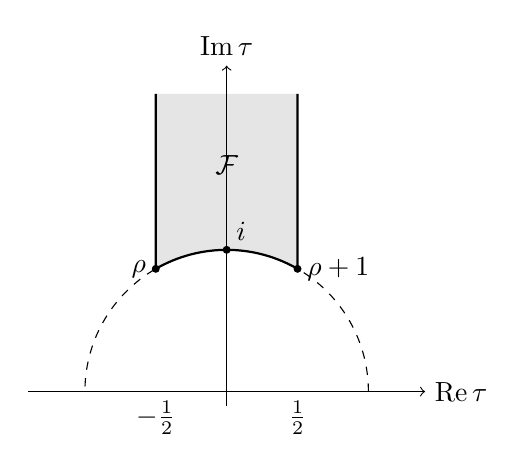
\begin{tikzpicture}[scale=1.8]
  \fill[gray!20] (-0.5,0.866) arc (120:60:1) -- (0.5,2.1) -- (-0.5,2.1) -- cycle;
  \draw[->] (-1.4,0)--(1.4,0) node[right]{$\mathrm{Re}\,\tau$};
  \draw[->] (0,-0.1)--(0,2.3) node[above]{$\mathrm{Im}\,\tau$};
  \draw[dashed] (1,0) arc (0:180:1);
  \draw[thick] (-0.5,2.1)--(-0.5,0.866) arc (120:60:1) -- (0.5,2.1);
  \fill (0,1) circle (0.8pt) node[above right]{$i$};
  \fill (-0.5,0.866) circle (0.8pt) node[left]{$\rho$};
  \fill (0.5,0.866) circle (0.8pt) node[right]{$\rho+1$};
  \node at (0,1.6) {$\mathcal{F}$};
  \node[below] at (-0.5,0) {$-\frac12$};
  \node[below] at (0.5,0) {$\frac12$};
\end{tikzpicture}
\end{center}
（$\mathrm{PSL}(2,\Z)=\SL(2,\Z)/\{\pm1\}$ である。）

\appJsol{I-13-4}
\begin{enumerate}
  \item $a=-1$, $b=0$：$4a^3+27b^2=-4\neq0$ で滑らか。$j=1728\cdot\dfrac{-4}{-4}=1728$。
  \item $a=0$, $b=1$：$4a^3+27b^2=27\neq0$ で滑らか。$j=1728\cdot0=0$。
  \item $a=-3$, $b=2$：$4a^3+27b^2=-108+108=0$。判別式が $0$ なので滑らかでなく、$j$ は定義されない（$j=\infty$ と見なす）。実際 $x^3-3x+2=(x-1)^2(x+2)$ で、点 $(1,0)$ がノードである（$y^2=(x-1)^2(x+2)$ の点 $(1,0)$ における（$x-1$, $y$ についての）最低次部分は $y^2-3(x-1)^2$ で、相異なる $2$ 本の接線をもつ）。
\end{enumerate}
（1）（2）は問題 I.13.3 の $j(i)=1728$, $j(\rho)=0$ に対応する曲線である。

\appJsol{I-14-1}
$d(g^{-1})=-g^{-1}\,dg\,g^{-1}$ より $g\,d(g^{-1})=-dg\,g^{-1}$ に注意する。$A$ は $1$ 形式なので、外微分を $A$ の右側に通すと符号が変わる。

\textbf{$dA'$ の計算.}
\[
  dA'=dg\wedge A\,g^{-1}+g\,dA\,g^{-1}-gA\wedge d(g^{-1})+dg\wedge d(g^{-1}).
\]
\textbf{$A'\wedge A'$ の計算.}
\begin{align*}
  A'\wedge A'&=gA\wedge Ag^{-1}+gA\,g^{-1}\wedge g\,d(g^{-1})+g\,d(g^{-1})\wedge gAg^{-1}+g\,d(g^{-1})\wedge g\,d(g^{-1})\\
  &=gA\wedge Ag^{-1}+gA\wedge d(g^{-1})-dg\wedge Ag^{-1}-dg\wedge d(g^{-1}).
\end{align*}
ここで第 $3$ 項に $g\,d(g^{-1})=-dg\,g^{-1}$ を、第 $4$ 項に $g\,d(g^{-1})\wedge g=-dg\,g^{-1}\wedge g=-dg$ を用いた。

\textbf{和.}
\begin{align*}
  F'&=dA'+A'\wedge A'\\
  &=\underbrace{(dg\wedge Ag^{-1}-dg\wedge Ag^{-1})}_{0}+g\,dA\,g^{-1}+\underbrace{(-gA\wedge d(g^{-1})+gA\wedge d(g^{-1}))}_{0}\\
  &\quad+\underbrace{(dg\wedge d(g^{-1})-dg\wedge d(g^{-1}))}_{0}+gA\wedge Ag^{-1}\\
  &=g\,(dA+A\wedge A)\,g^{-1}=gFg^{-1}.
\end{align*}
（別解：共変微分 $D=d+A$ について $D'=gDg^{-1}$ であり、$F=D^2$ なので $F'=D'^2=gD^2g^{-1}=gFg^{-1}$。）曲率は随伴表現で共変的に変換するので、$\Tr F^k$ はゲージ不変であり、Chern 類（特性類）を定める。

\appJsol{I-14-2}
\begin{enumerate}
  \item $d\phi$ は極 $\theta=0,\pi$ で特異だが、$\theta\to0$ で $1-\cos\theta\sim\theta^2/2$ となり、$\theta^2d\phi=x\,dy-y\,dx$（$x=\theta\cos\phi$, $y=\theta\sin\phi$ は北極の近くの局所座標）は滑らか。よって $A_N$ は北極を含む $U_N$ 上で滑らか。同様に $\theta\to\pi$ で $1+\cos\theta\to0$ となり、$A_S$ は南極を含む $U_S$ 上で滑らか。
  \item 重なり（赤道付近）で
  \[
    A_N-A_S=\frac n2\bigl[(1-\cos\theta)+(1+\cos\theta)\bigr]d\phi=n\,d\phi=d(n\phi).
  \]
  よって $\lambda=n\phi$。ゲージ変換 $e^{i\lambda}=e^{in\phi}$ が赤道上で一価（$\phi\mapsto\phi+2\pi$ で不変）であるためには $e^{2\pi in}=1$、すなわち $n\in\Z$ が必要。これが Dirac の量子化条件である。
  \item $F=dA_N=\dfrac n2\sin\theta\,d\theta\wedge d\phi$（$U_S$ 上でも $dA_S$ は同じ式）。
  \[
    \frac1{2\pi}\int_{S^2}F=\frac1{2\pi}\cdot\frac n2\int_0^{\pi}\sin\theta\,d\theta\int_0^{2\pi}d\phi=\frac1{2\pi}\cdot\frac n2\cdot2\cdot2\pi=n.
  \]
  あるいは Stokes の定理で $\int_{S^2}F=\int_{\text{北}}dA_N+\int_{\text{南}}dA_S=\oint_{\text{赤道}}(A_N-A_S)=2\pi n$。
\end{enumerate}
第 $1$ Chern 数 $n$ はモノポールの磁荷であり、$S^2$ 上の直線束 $\OO(n)$（の位相型）を分類する。

\appJsol{I-14-3}
Kodaira 分類（の F 理論で用いる部分）を表にまとめる：
\[
\begin{array}{c|c|c|c|c}
  \mathrm{ord}f & \mathrm{ord}g & \mathrm{ord}\Delta & \text{ファイバー型} & \text{ゲージ代数}\\\hline
  0 & 0 & n & I_n & \mathfrak{su}(n)\\
  \geq1 & 1 & 2 & II & -\\
  1 & \geq2 & 3 & III & \mathfrak{su}(2)\\
  \geq2 & 2 & 4 & IV & \mathfrak{su}(3)\\
  \geq2 & \geq3 & 6 & I_0^* & \mathfrak{so}(8)\\
  2 & 3 & n+6 & I_n^* & \mathfrak{so}(2n+8)\\
  \geq3 & 4 & 8 & IV^* & \mathfrak{e}_6\\
  3 & \geq5 & 9 & III^* & \mathfrak{e}_7\\
  \geq4 & 5 & 10 & II^* & \mathfrak{e}_8
\end{array}
\]
\begin{enumerate}
  \item $\Delta=4z^{12}+27z^{10}=z^{10}(27+4z^2)$。$(\mathrm{ord}f,\mathrm{ord}g,\mathrm{ord}\Delta)=(4,5,10)$ で $II^*$、$\mathfrak{e}_8$。
  \item $\Delta=4z^9+27z^{10}=z^9(4+27z)$。$(3,5,9)$ で $III^*$、$\mathfrak{e}_7$。
  \item $\Delta=4(-3)^3+27(2+z^n)^2=-108+27(4+4z^n+z^{2n})=108z^n+27z^{2n}$。$(0,0,n)$ で $I_n$、$\mathfrak{su}(n)$。$f,g$ が $0$ にならないのに $\Delta$ が消えるのは、$x=1$ で $x^3-3x+2=(x-1)^2(x+2)$ のノードが現れるからである（問題 I.13.4(3)）。
  \item $\Delta=4(-3z^2)^3+27(2z^3+z^4)^2=-108z^6+27(4z^6+4z^7+z^8)=108z^7+27z^8$。$(2,3,7)$ で $I_1^*$、$\mathfrak{so}(10)$。
\end{enumerate}
（実際のゲージ代数はモノドロミーによって $\mathfrak{sp}$ や $\mathfrak{so}(2n+7)$、$\mathfrak{f}_4$、$\mathfrak{g}_2$ などに折りたたまれることがある。ここでは分裂型を仮定した。）

% ==========================================================
\section{発展問題の解答・解説}

\appJsol{I-2-5}
$\m\cap\Z=0$ と仮定して矛盾を導く。$K=\Z[x]/\m$ は体で、$\Z\to K$ は単射なので $\Q\subset K$。$\alpha$ を $x$ の像とすると $K=\Z[\alpha]$。

\textbf{$\alpha$ は $\Q$ 上代数的.} そうでなければ $\Z[\alpha]\cong\Z[x]$ となり、これは体でない。よって $a_n\alpha^n+\dots+a_0=0$（$a_i\in\Z$, $a_n\neq0$）なる関係がある。

\textbf{整拡大.} $B=\Z[1/a_n]\subset K$ とすると、両辺を $a_n$ で割って $\alpha$ は $B$ 上モニック多項式の根、すなわち $B$ 上整。よって $K=B[\alpha]$ は $B$ 上整。

\textbf{補題.} $B\subset K$ が整拡大で $K$ が体なら $B$ は体。（$0\neq b\in B$ に対し $b^{-1}\in K$ は $B$ 上整なので $b^{-m}+c_1b^{-m+1}+\dots+c_m=0$、$c_i\in B$。両辺に $b^{m-1}$ を掛けて $b^{-1}=-(c_1+c_2b+\dots+c_mb^{m-1})\in B$。）

\textbf{矛盾.} 補題より $\Z[1/a_n]$ は体である。しかし $a_n$ を割り切らない素数 $p$ をとると、$\Z[1/a_n]$ の元は $m/a_n^k$ の形なので $1/p\notin\Z[1/a_n]$。よって $\Z[1/a_n]$ は体でない。矛盾。

\textbf{解説.} この結果と $\Z[x]/(p)\cong\F_p[x]$ が PID であることを合わせると、$\Z[x]$ の極大イデアルは $(p,f)$（$f$ は $\bmod p$ で既約な多項式）の形に限ることがわかる。$\Spec\Z[x]$ は「$\Spec\Z$ 上の $\A^1$」であり、その閉点はすべてどこかの素数 $p$ 上のファイバー $\A^1_{\F_p}$ に乗っている。$p$ 方向と $x$ 方向の $2$ 次元からなる「算術曲面」という見方ができる。これは Hilbert の零点定理の算術版（$\Z$ は Jacobson 環）の一例である。

\appJsol{I-6-5}
\begin{enumerate}
  \item 問題 I.5.1 より $k[C]\cong k[x]$（$y\mapsto x^2$）で、原点は極大イデアル $(x)$ に対応する。よって $\OO_{C,0}\cong k[x]_{(x)}=\{f/g\mid g(0)\neq0\}$。$0\neq h=f/g$ について、$f=x^nf_1$（$f_1(0)\neq0$）と書けば $h=(f_1/g)x^n$ で、$u=f_1/g$ は $u(0)\neq0$ なので単元。$n$ は $f$ の $0$ での零点の位数なので一意。よって $\OO$ は $x$ を一意化元とする離散付値環。
  \item $v(x)=1$。$y=x^2$ なので $v(y)=2$。$y-ax=x^2-ax=x(x-a)$ で $x-a$ は $0$ で $-a\neq0$ なので単元。よって $v(y-ax)=1$。
  \item 直線 $\ell=\{h=0\}$ と $C$ の原点での交点数は $\dim_k\OO_{C,0}/(h)=v(h)$ である（DVR では $(h)=(x^{v(h)})$ で、$\OO/(x^n)$ は $n$ 次元）。
  \begin{itemize}
    \item $y=0$（$x$ 軸）：$v(y)=2$。$x$ 軸は原点での $C$ の接線なので交点数 $2$。
    \item $x=0$（$y$ 軸）：$v(x)=1$。横断的に交わり交点数 $1$。
    \item $y=ax$ ($a\neq0$)：$v=1$。横断的で交点数 $1$。もう一つの交点は $x=a$ の点 $(a,a^2)$ で、合計 $2$ が Bézout の数（射影化したときの $2\cdot1$）と一致する。
  \end{itemize}
\end{enumerate}
\textbf{解説.} 滑らかな曲線上の点の局所環は DVR であり、付値が「その点での零点・極の位数」を測る。これが因子 $\mathrm{div}(f)=\sum v_P(f)P$ の定義の基礎になる。

\appJsol{I-7-6}
チャート $y=tx$（座標 $(x,t)$）で $f=y^2-x^3-x^2$ を引き戻すと
\[
  t^2x^2-x^3-x^2=x^2\bigl(t^2-x-1\bigr).
\]
因子 $x^2$ は例外因子 $E=\{x=0\}$（原点の逆像）を $2$ 重に表す（原点の重複度が $2$ であることに対応）。これを除いた固有変換は
\[
  \widetilde C:\ t^2=x+1.
\]
$g=t^2-x-1$ の勾配 $(g_x,g_t)=(-1,2t)$ は決して $0$ にならないので、$\widetilde C$ は（このチャートで）滑らか。$\widetilde C\cap E$ は $x=0$, $t^2=1$ より $t=\pm1$ の $2$ 点。

もう一つのチャート $x=sy$（座標 $(s,y)$）では $f=y^2-s^3y^3-s^2y^2=y^2(1-s^2-s^3y)$。固有変換は $1-s^2-s^3y=0$ で、$s=0$ は $1=0$ となり $\widetilde C$ 上にないので、勾配の $y$ 成分 $-s^3\neq0$ より滑らか。$E=\{y=0\}$ との交点は $s=\pm1$ で、$s=1/t$ により上の $2$ 点と同じ点である。

\textbf{解説.} $t=y/x$ は原点に近づく方向の傾きであり、$t=\pm1$ は接錐 $y=\pm x$（問題 I.7.1）の $2$ 本の接線に対応する。ブローアップは原点を「接方向の集合 $\PP^1$」に置き換える操作であり、ノードの $2$ つの枝は異なる接方向をもつので $\widetilde C$ 上では $2$ 点に分離され、特異点が解消される。$\widetilde C$ は $t$ を座標として $\A^1$ に同型であり（$x=t^2-1$, $y=t(t^2-1)$）、これはノード曲線の有理パラメータ表示を与えている。

\appJsol{I-9-5}
\begin{enumerate}
  \item \textbf{核.} $\exp(2\pi if)=1$ なる正則関数 $f$ は値が整数で連続、したがって局所定数な整数値関数。よって $\Ker=\underline\Z$ で、$\underline\Z\to\OO_X$ は単射。

  \textbf{茎での全射性.} $g\in\OO_{X,p}^*$ を $p$ の近くで消えない正則関数とする。$p$ を中心とする十分小さい円板 $D$ 上で $g(D)$ は $0$ を含まない円板に含まれるので、そこで $\log$ の分枝がとれ、$f=\frac1{2\pi i}\log g$ は $D$ 上正則で $\exp(2\pi if)=g$。よって茎の写像は全射であり、層の射として全射。茎ごとに完全なので層の完全系列である。
  \item $z\in\OO_X^*(X)$ を考える。$\exp(2\pi if)=z$ なる $f\in\OO_X(X)$ があれば $L=2\pi if$ は $e^L=z$ を満たす大域的な対数となり、問題 I.9.3(2) に反する。よって大域切断の写像は全射でない。
\end{enumerate}
\textbf{解説.} 層の短完全系列から得られる長完全系列
\[
  0\to H^0(X,\underline\Z)\to H^0(X,\OO)\to H^0(X,\OO^*)\xrightarrow{\ \delta\ }H^1(X,\underline\Z)\to H^1(X,\OO)\to\cdots
\]
において、大域切断の全射性のずれは連結写像 $\delta$ の像、すなわち $H^1(X,\underline\Z)\cong H^1(\C^*,\Z)\cong\Z$ で測られる。$\delta(g)$ は $g$ の巻き数 $\frac1{2\pi i}\oint dg/g$ であり、$\delta(z)=1$。問題 I.9.3(1) の「上で $0$、下で $2\pi i$」というずれ（を $2\pi i$ で割ったもの）が、まさにこの Čech コホモロジー類の代表元である。同じ系列をコンパクトな多様体に適用すると $\Pic X=H^1(X,\OO^*)\to H^2(X,\Z)$ が直線束の第 $1$ Chern 類を与え、物理ではモノポールの磁荷（問題 I.14.2）に対応する。

\appJsol{I-10-5}
$k$ 代数準同型 $\phi:k[x,y]\to k[\varepsilon]$ は $\phi(x)=a+u\varepsilon$, $\phi(y)=b+v\varepsilon$ の $4$ つの値で決まり、$\phi$ が $A=k[x,y]/(f)$ を経由することは $\phi(f)=0$ と同値である。$\varepsilon^2=0$ なので Taylor 展開は $1$ 次で打ち切られ、
\[
  f(a+u\varepsilon,\ b+v\varepsilon)=f(a,b)+\bigl(f_x(a,b)\,u+f_y(a,b)\,v\bigr)\varepsilon.
\]
これが $0$ であることは $f(a,b)=0$ かつ $f_x(a,b)u+f_y(a,b)v=0$ と同値。よって主張の一対一対応を得る。

\textbf{解釈.} $(a,b)$ は曲線 $C=\Zero(f)$ 上の点（$\Spec k[\varepsilon]$ の唯一の点の像）、$(u,v)$ は条件 $\nabla f(a,b)\cdot(u,v)=0$ を満たすベクトル、すなわち $(a,b)$ における Zariski 接空間 $T_{(a,b)}C$ の元である。つまり $\Spec k[\varepsilon]\to C$ は「点と、その点での接ベクトル」の組と同じものである。$\Spec k[\varepsilon]$ は「$1$ 点とそこから出る無限小の矢印」と思える。

\textbf{ノードの原点.} $f=y^2-x^3-x^2$ では $f_x(0,0)=f_y(0,0)=0$ なので、$(u,v)$ に条件はつかず、原点での接ベクトルは $k^2$ 全体で $2$ 次元。曲線は $1$ 次元なのに接空間が $2$ 次元であることが、原点が特異点であることを表している（問題 I.6.4 と整合）。非特異点では $\nabla f\neq0$ なので接空間は $1$ 次元になる。

\appJsol{I-11-6}
$X=E$（$g=1$）、$Y=\C P^1$（$g=0$）、$\deg\wp=2$ として Riemann--Hurwitz を用いると
\[
  2\cdot1-2=2(2\cdot0-2)+\sum_p(e_p-1)\quad\Longrightarrow\quad\sum_p(e_p-1)=4.
\]
次数 $2$ なので $e_p\in\{1,2\}$、よって分岐点（$e_p=2$）はちょうど $4$ 個。
\begin{itemize}
  \item $z=0$：$\wp$ は $2$ 位の極をもつので、$\infty$ の上で $e_0=2$。
  \item 半周期 $\omega\in\{\tfrac12,\tfrac\tau2,\tfrac{1+\tau}2\}$：$\wp$ は偶関数なので $\wp'$ は奇関数で周期的。$2\omega\in\Lambda$ より
  \[
    \wp'(\omega)=\wp'(\omega-2\omega)=\wp'(-\omega)=-\wp'(\omega)
  \]
  で $\wp'(\omega)=0$。よって $e_\omega\geq2$、すなわち $e_\omega=2$。
\end{itemize}
これで $4$ 個がすべて見つかった。分岐値は $\infty$ と $e_i=\wp(\omega_i)$ ($i=1,2,3$) である。

\textbf{解説.} $x=\wp(z)$, $y=\wp'(z)$ とおくと $y^2=4x^3-g_2x-g_3=4(x-e_1)(x-e_2)(x-e_3)$ が成り立つ。$(x,y)\mapsto x$ が $\wp$ に対応する $2$ 重被覆で、$y=0$ となる $3$ 点 $x=e_i$ と無限遠点 $x=\infty$ の $4$ 点で分岐する。逆に、$\C P^1$ の $4$ 点で分岐する $2$ 重被覆は種数 $1$ の曲線であり、$4$ 点の交差比が $j$ 不変量を決める。

\appJsol{I-12-5}
\begin{enumerate}
  \item 随伴公式を $2$ 回用いて $K_X\cong\OO_{\PP^5}(-6+3+3)|_X=\OO_X$。よって $c_1(X)=0$。
  \item $H^4=0$ として展開する：
  \begin{align*}
    (1+H)^6&=1+6H+15H^2+20H^3,\\
    (1+3H)^{-2}&=1-6H+27H^2-108H^3.
  \end{align*}
  （$(1+u)^{-2}=1-2u+3u^2-4u^3+\cdots$ に $u=3H$ を代入。）積は
  \begin{align*}
    c_1&=6-6=0,\\
    c_2&=15-36+27=6,\\
    c_3&=20+15\cdot(-6)+6\cdot27+(-108)=20-90+162-108=-16.
  \end{align*}
  $\int_XH^3=3\cdot3=9$（$X$ は $\PP^5$ の $3$ 平面と $3\cdot3$ 点で交わる）より
  \[
    \chi(X)=-16\cdot9=-144.
  \]
  \item $6$ 変数の $3$ 次単項式は $\binom{8}{3}=56$ 個で、$2$ つの $3$ 次式 $(f_1,f_2)$ のパラメータは $112$。同じ $X$ を与える変換は、$(f_1,f_2)$ の一次結合の取り替え $\GL(2)$（次元 $4$）と座標変換 $\GL(6)$（次元 $36$）。ただしスカラー倍 $x\mapsto\lambda x$ は $(f_1,f_2)\mapsto\lambda^3(f_1,f_2)$ を引き起こし、$\GL(2)$ のスカラー倍と重複するので $1$ 次元分を足し戻す：
  \[
    h^{2,1}=112-4-36+1=73.
  \]
  $h^{1,1}=1$（Lefschetz の超平面定理）と合わせて $\chi=2(1-73)=-144$ で、（2）と一致する。
\end{enumerate}
\textbf{解説.} 完全交差 CY の一般論として、$\PP^{n}$ の次数 $(d_1,\dots,d_r)$ の完全交差は $\sum d_i=n+1$ のとき CY である。$3$ 次元では quintic $(5)$、$(2,4)\subset\PP^5$、$(3,3)\subset\PP^5$、$(2,2,3)\subset\PP^6$、$(2,2,2,2)\subset\PP^7$ の $5$ 種類があり、Euler 数はそれぞれ $-200,-176,-144,-144,-128$ である。

\appJsol{I-13-5}
\begin{enumerate}
  \item $\sigma(x,y)=(-x,\ iy)$ とする。$(iy)^2=-y^2=-(x^3-x)=(-x)^3-(-x)$ なので $\sigma$ は $E_1$ を保ち、無限遠点 $O$ を固定する。$\sigma^2(x,y)=(x,-y)$ は $[-1]$（反転）、$\sigma^4=\mathrm{id}$ なので位数 $4$。
  \item $\tau(x,y)=(\rho x,\ -y)$ とする。$(-y)^2=y^2=x^3+1=(\rho x)^3+1$ なので $E_2$ を保つ。$\rho x$ の部分は位数 $3$、$-y$ の部分は位数 $2$ なので $\tau$ の位数は $6$。
  \item $\SL(2,\Z)$ の中で $\tau\in\mathbb H$ を固定する元を数える。
  \begin{itemize}
    \item 一般の $\tau$：$\pm1$ のみ（位数 $2$）。これは任意の楕円曲線の自己同型 $[-1]:(x,y)\mapsto(x,-y)$ に対応。
    \item $\tau=i$：$\{\pm1,\pm S\}$（位数 $4$、$S^2=-1$）。$E_1$（$j=1728$）の $\Z/4$ に対応。
    \item $\tau=\rho$：$\{\pm1,\pm ST,\pm(ST)^2\}$（位数 $6$、$(ST)^3=-1$）。$E_2$（$j=0$）の $\Z/6$ に対応。
  \end{itemize}
\end{enumerate}
\textbf{解説.} 楕円曲線 $E_\tau$ の自己同型群は、$\tau$ の $\SL(2,\Z)$ での固定部分群と一致する（$\pm1$ は全点を固定するので $\mathrm{PSL}(2,\Z)$ で見ると一般の点の固定群は自明）。$\mathcal M_{1,1}=\mathbb H/\SL(2,\Z)$ は粗モジュライ空間としては $j$ により $\A^1$ と同一視されるが、$j=1728$ と $j=0$ に余分な対称性 $\Z/2$, $\Z/3$（$\mathrm{PSL}$ で見て）をもつオービフォールド点がある。この「点ごとに自己同型群が異なる」ことが、$\mathcal M_{1,1}$ が良いモジュライ空間（普遍族をもつ空間）にならず、スタックとして扱う必要がある理由である。オービフォールド Euler 数は $\chi(\mathcal M_{1,1})=-\tfrac1{12}$ であり、これは弦理論の $1$ ループ分配関数の計算などに現れる。

\appJsol{I-14-4}
\begin{enumerate}
  \item $F=\sum w_i^2-\varepsilon$ の勾配は $2(w_1,\dots,w_4)$ で、$0$ になるのは $w=0$ のみ。$\varepsilon\neq0$ なら $0\notin X_\varepsilon$ なので $X_\varepsilon$ は滑らか。$\varepsilon=0$ なら $0\in X_0$ で、原点が唯一の特異点（コニフォールド特異点、$\Sigma w_i^2=0$ は $3$ 次元の $2$ 次錐）。
  \item $w\in\R^4$ なら方程式は $\sum w_i^2=\varepsilon$ となり、半径 $R=\sqrt\varepsilon$ の $3$ 次元球面。（一般に $w=x+iy$ と書くと $X_\varepsilon$ は $|x|^2-|y|^2=\varepsilon$, $x\cdot y=0$ となり、$y$ を $x\in S^3$ での接ベクトルと見て $X_\varepsilon\cong T^*S^3$ となる。$S$ はその零切断である。）

  半径 $R$ の $S^3$ の体積は $2\pi^2R^3$ なので
  \[
    \mathrm{Vol}(S)=2\pi^2\varepsilon^{3/2}.
  \]
  \item $S$ 上では $w_i=x_i$ は実で、$\Omega|_S=dx_1\wedge dx_2\wedge dx_3/x_4$。$S$ を上半球 $x_4>0$ と下半球 $x_4<0$ に分け、$(x_1,x_2,x_3)$ を半径 $\sqrt\varepsilon$ の球体 $B$ 上の座標として用いる。上半球では $x_4=\sqrt{\varepsilon-r^2}$（$r^2=x_1^2+x_2^2+x_3^2$）なので
  \[
    \int_{\text{上}}\Omega=\int_B\frac{d^3x}{\sqrt{\varepsilon-r^2}}=4\pi\int_0^{\sqrt\varepsilon}\frac{r^2\,dr}{\sqrt{\varepsilon-r^2}}.
  \]
  $r=\sqrt\varepsilon\sin\theta$ と置換すると
  \[
    \int_0^{\sqrt\varepsilon}\frac{r^2\,dr}{\sqrt{\varepsilon-r^2}}=\varepsilon\int_0^{\pi/2}\sin^2\theta\,d\theta=\frac{\pi\varepsilon}{4}
  \]
  なので $\int_{\text{上}}\Omega=\pi^2\varepsilon$。下半球では $x_4<0$ で被積分関数の符号が変わるが、$S$ の向き（$\R^4$ の球面としての向き）に関して $(x_1,x_2,x_3)$ の向きも逆転するので、寄与は同じく $\pi^2\varepsilon$。よって
  \[
    \int_S\Omega=2\pi^2\varepsilon\qquad(\text{向きを逆にとれば }-2\pi^2\varepsilon).
  \]
  検算：$w\mapsto\lambda w$ ($\lambda=\sqrt\varepsilon$) は $X_1\to X_\varepsilon$ の同型で、$\Omega$ は $\lambda^3/\lambda=\lambda^2=\varepsilon$ 倍される。よって周期は $\varepsilon$ に比例し、$\varepsilon=1$ での値 $2\pi^2$（単位 $S^3$ の体積）に一致する。

  （$\Omega$ を $\sum w_i^2-\varepsilon$ の留数 $\Res\dfrac{d^4w}{F}=\dfrac{dw_1\wedge dw_2\wedge dw_3}{\partial F/\partial w_4}=\dfrac{dw_1\wedge dw_2\wedge dw_3}{2w_4}$ で正規化すれば周期は $\pi^2\varepsilon$ になる。）
  \item $\varepsilon\to0$ で $S^3$（「消滅サイクル」）は体積 $\varepsilon^{3/2}\to0$ で潰れ、$X_\varepsilon$ は特異なコニフォールド $X_0$ に退化する。周期 $z=\int_S\Omega\propto\varepsilon$ は複素構造モジュライ空間のこの点の近くでの自然な座標であり、$z=0$ はモジュライ空間の「コニフォールド点」である。

  タイプ IIB 弦理論では、D3 ブレーンを $S^3$ に巻き付けた状態は質量 $\propto|z|$ の BPS 粒子（ブラックホール）となり、$z\to0$ で質量ゼロになる。これを有効理論に含めると、プレポテンシャルの $z^2\log z$ 型の特異性（$S^3$ と双対なサイクル上の周期が $\frac{z}{2\pi i}\log z$ のように振る舞い、$z\mapsto e^{2\pi i}z$ で $S^3$ のサイクル分ずれる Picard--Lefschetz モノドロミー）が、質量ゼロの粒子を積分した効果として説明される（Strominger）。さらに、$S^3$ を潰した後に別の $S^2$ を膨らませる操作（コニフォールド転移）によって、トポロジーの異なる CY 多様体の間を連続的に移ることができる。
\end{enumerate}
